% !TEX root =  ../FinalReport.tex

\chapter{Project Management}
\label{sec:ProjectManagement}

To ensure a smooth development process, all research and implementation was planned ahead of time.
This chapter details these plans including a complete schedule, the development methodology used, the tools used, and the potential risks and associated contingencies.

\section{Software Development Methodology}
Plan-driven solutions depend on a rigid specification being completed before development\cite{modules:CS261}, which did not fit with the more abstract goals of the visualization portion.
Additionally, some of the main advantages of plan-driven approaches only apply when introducing new team members and handling large teams.
Neither scenario applies here, as only one person is undertaking active development.

For these reasons, an Agile approach was taken with a development cycle completing every two weeks.
The goals for each development cycle were documented using Trello.
It was planned that the supervisor would be contacted every week with the current status of the project and the progress made in the current cycle.
These contacts would either take place over e-mail if there were no pressing questions to ask, and otherwise take place on Microsoft Teams.
Unfortunately, this did not happen for the first few weeks, as other work was vying for attention and preventing project work from taking place.
This was resolved in Week 5, and there is now frequent email correspondence.

\section{Project Timeline}
The project was split into multiple tasks to schedule it effectively.
These tasks are scheduled on both a Gantt Chart in \cref{fig:project schedule gantt}, and as a table in \cref{tab:project schedule table}.
The timeline has been well followed, and this schedule has been left unchanged over the course of the project. 
Over the Christmas break no work was scheduled, to allow time to be spent on other assignments.%time on the other courseworks the researcher will have due.

The development of the visualization was scheduled concurrently with optimizing the simulation, in case some strides in visualization required extra optimizations to run in real-time.
While not strictly required, some optimizations were developed in this time to push performance further.
% This was not strictly the case, but some optimizations were developed in this time period to push performance further.
A Code Freeze was set for Week 22, to focus the researcher entirely on the presentation.
%where development is then completely focused on the presentation.

\begin{figure}[ht]
    \centering
    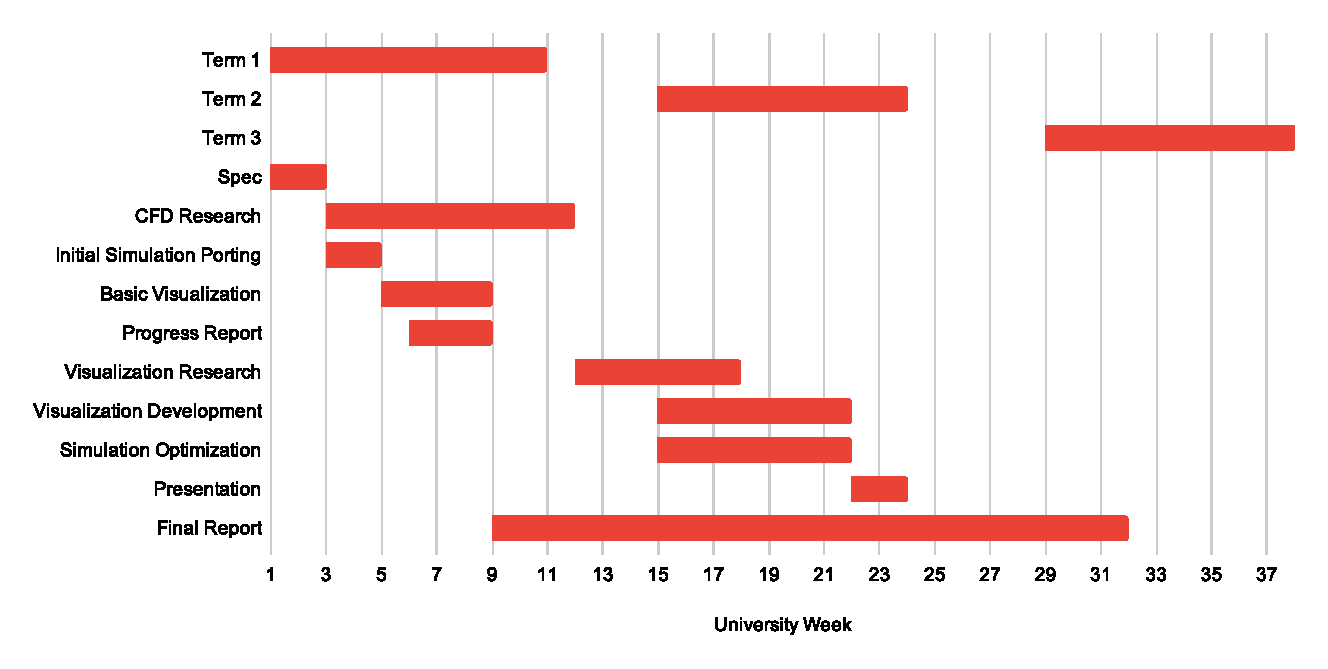
\includegraphics[width=\linewidth]{Ch50ProjectManagement/cs311_gantt_chart.svg.pdf}
    \caption{Project Schedule as a Gantt Chart}
    \label{fig:project schedule gantt}
\end{figure}

\begin{table}[ht]
    \centering
    \begin{tabular}{l|c|c}
    \textbf{Task} & \textbf{Start Week} & \textbf{End Week} \\
    \hline
    Spec & 1 & 3 \\
    CFD Research & 3 & 12 \\
    Initial Simulation Porting & 3 & 5 \\
    Basic Visualization & 5 & 9 \\
    Progress Report & 6 & 9 \\
    Visualization Research & 12 & 18 \\
    Visualization Development & 15 & 22 \\
    Simulation Optimization & 15 & 22 \\
    Presentation & 22 & 24 \\
    Final Report & 9 & 32 \\
    \end{tabular}
    \caption{Project Schedule Tasks}
    \label{tab:project schedule table}
\end{table}

\section{Tools}
\label{sec:ProjManagementTools}
\shell{gcc 8} was used to compile the program.
This version had stable support for the C++14 and C++17 standards, allowing modern techniques to be used in the program.
CMake was used to handle building the program source files.
Versions 3.8 and up support CUDA as a first-class language, which simplified the compilation process.
% The CLion IDE is used on the researcher's personal machine, as the researcher is familiar with the other IDEs in this family.
% If DCS machines are used, GNU Emacs will be used to edit files instead.

Git was used for source control, synchronized to a private GitHub repository to avoid data loss.
The researcher used the CLion IDE to develop the program, which simplified building the program and interacting with source control.

\LaTeX{} was used to create the various reports and non-program deliverables required by the project, which were hosted on Overleaf so they could be compiled on Windows and Linux without installing a \LaTeX{} environment.

%Trello
Trello was used to track bugs and upcoming features in each development cycle.
Google Drive was used to host other documents, e.g. scanned notes, that were created during development.

\section{Risk Management}
% As the project continues, there are risks that may impede progress and even prevent the project from succeeding.
When progressing through the project, there were risks that could impede progress and even prevent the project from succeeding.
Being aware of these risks allowed them to be predicted ahead of time, avoided, or in the worst case mitigated once they arrived.
Risk can be calculated with the following equation, where Severity and Likelihood are graded between 1 and 5.
\begin{equation*}
    Risk = Severity * Likelihood
\end{equation*}

Of these risks, Illness and Other Pressures were encountered during development.
Both were mitigated quickly and did not cause a large delay.
% Some of these risks were encountered, including a new risk (Other Pressures) which was not accounted for in the Specification.
% Thankfully this risk did not cause a large delay.

\subsection{Misscheduling}
It may have been possible that the features outlined in \cref{sec:Requirements} were too great to be implemented in the allotted time.
In that case, the quality of work could have to be reduced to meet deadlines, or the schedule would need to be changed.
This is especially relevant to the Visualization portion of the project, which was not fully planned until the research was completed.

\textbf{Risk} = 2 * 2 = 4

\textbf{Avoidance:}
Previous projects were used as a reference to predict how long implementing features will take, and inform the schedule.
As new Visualization features were discussed, the impact on scheduling they each have were considered.

\textbf{Contingency:}
The scope of the project could have been reduced to allow the report to be completed in time.
A ``code freeze'' was implemented close to the presentation deadline to ensure enough time is spent polishing the presentation and report.

\subsection{Other Pressures}
While the project schedule may have been well estimated based on the work required for the project, the amount of work required for other modules was larger than expected.
This manifested in Term 1, where the researcher took more modules than usual. 
Additionally, the removal of in-person lectures due to COVID-19 led to a lack of overall structure, which made organizing the other work more difficult.
This did not impact the schedule.

\textbf{Risk} = 2 * 1 = 2

\textbf{Avoidance:}
% A more balanced set of modules between Term 1 and Term 2 could have helped resolve this, however on the other side of the coin the researcher had fewer modules in Term 2.
% Balancing modules between Term 1 and Term 2 could have resolved this, but as Term 2 had fewer mo
% Next term the researcher will try to maintain a schedule for working on other module content, which should make up for a lack of in-person lectures.
This could have been avoided by better balancing the modules between Term 1 and Term 2, but on the flip-side having fewer modules in Term 2 allowed for more project work to be completed.

\textbf{Contingency:}
As before, the scope of the project could have been reduced to allow the report to be completed in time.
If module work took more time than expected by week 20, the code freeze could have been pulled forwards to week 20 or 21 to spend more time on the presentation.


\subsection{Loss of Hardware Access}
As noted in \cref{sec:Requirements_HardwareSoftware}, a GPU is required for the project to be tested and developed.
The main development environment was the researcher's personal computer, which has a suitable GPU.
However, if this computer were to break down or be stolen, there was no readily available alternate environment.
Under normal circumstances the Department of Computer Science labs would be used instead, as they also have suitable GPUs, but the virus situation prevented this.

\textbf{Risk} = 5 * 1 = 5

\textbf{Avoidance:}
Not possible.

\textbf{Contingency:}
Student insurance could have been used to purchase a new GPU/computer if it is stolen.
Failing this, the DCS clusters could be used, but these would likely have high contention from other students who need to use GPUs remotely.

\subsection{Illness}
It is always prudent to consider the possibility that the stakeholders may fall ill and be unable to work on the project for some time.
This was exacerbated by the situation with COVID-19, making potential illnesses more dangerous than usual.

This risk manifested during Week 7 and delayed work on the project by three days.
However the bulk of the current work had been completed by that point, so this module was not affected.%other modules were affected.

\textbf{Risk} = 4 * 2 = 8

\textbf{Avoidance:}
Not possible.

\textbf{Contingency:}
The schedule would need to be changed to account for the lack of time spent working.
Some requirements could be reduced or removed entirely.

